\section{Introduction} \label{sec:introduction}

% What are containers and why they are becoming popular: pointing out portability and resource efficiency.

Containerization is a critical trend of applications running in data centers.
By wrapping a process into a complete filesystem and namespace cell, a container
has everything needed to run the process, including executables, libraries, system
tools, configurations, etc., without relying on external dependencies. 
Therefore, one container
is highly portable to run on any host with a proper OS kernel, and independent
with other containers on the same host without naming or version conflicts.
Such portability and independence significantly simplifies the life cycle of
a containerized application, from testing to high availability maintenance.

Ideally, containers should also have good performance and resource efficiency,
since they can directly run on bare-metal hosts without the overhead to run
hypervisor and guest OS in traditional visualization. However, perhaps 
surprisingly, we find measured evidence of significant bottlenecks in the 
network-level performance of containerized applications. We set up two iPerf containers running in server and client roles respectively and benchmark the network bandwidth between them when they use three different networking modes:
\begin{itemize}
	\item {\em Host}, in which one container binds an interface
and a port on the host and use the host's IP to communicate, like an ordinary
process.
	\item {\em Bridge}, in which all containers on the same host are connected to a common network bridge in OS kernel. It is only used for
	intra-host communications.  
	\item {\em Overlay}, in which each host runs a software router which
	connects all containers on the host via bridge network. An overlay 
	network crossing multiple hosts is constructed by the software routers
	to achieve a uniform IP assignment and traffic routing on the overlay.
\end{itemize}

\begin{figure}[ht]
     \centering 
     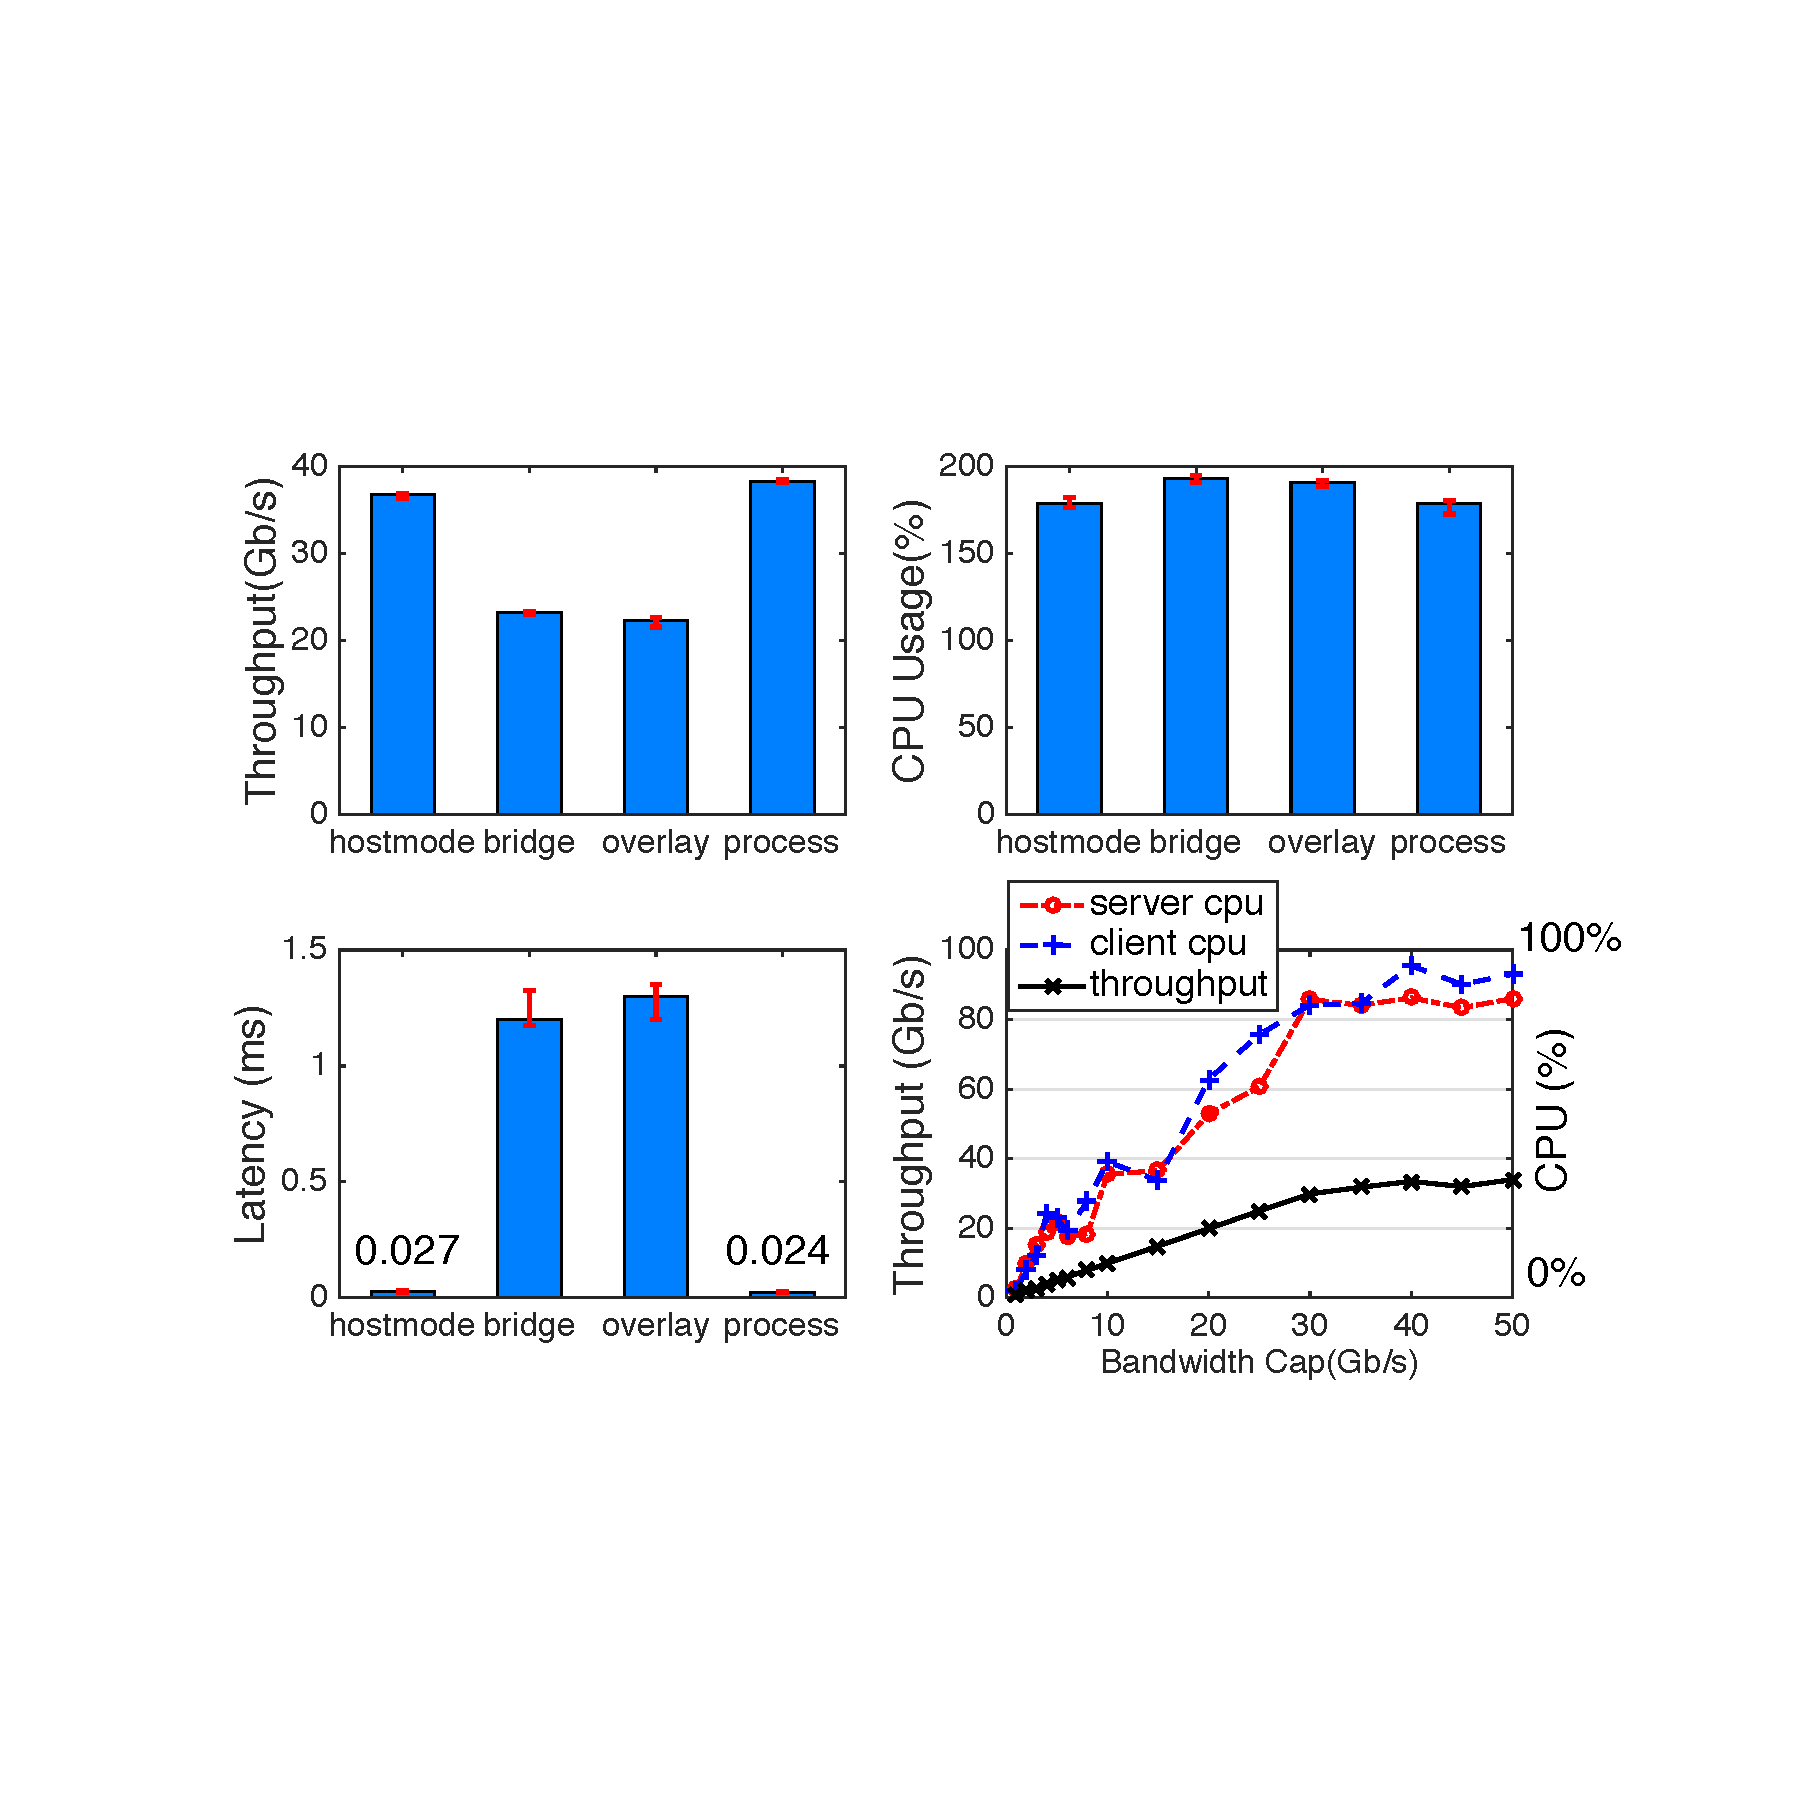
\includegraphics[width=0.5\textwidth]{figures/intro/intro_exist.pdf} 
     \label{fig:intro_exist}
     \caption{The measurement on existing solutions.} 
\end{figure} 

Figure XXX shows
the network bandwidth between two containers running on bare-metal hosts with 
Intel XXX CPU and Mellanox YYY NIC (40Gbps speed). Figure XXX (a) benchmarks
three available networking modes when two containers are located in the same 
host. Host mode has a throughput close to raw processes, while both bridge
and overlay modes has a XXX\% throughput drop due to the overhead to 
process packets in the host OS kernel. While the throughputs of all the three
network modes are XXX\% lower than the NIC speed and YYY\& lower than the memory
speed, Figure XXX (b) explains that the bottleneck is on CPU, since both
the sender and the receiver saturate a CPU core for just processing the traffic.
The results are similar when the two containers are on different hosts, as shown
in Figure YYY. The bad performance and high CPU overhead inherently from 
the TCP/IP stack used for inter-connecting containers. TCP/IP split data into 
packets and each packet can generate numerous system calls, interrupts, task 
switches and data coping, etc., which cost tremendous CPU cycles.

The inefficiency of current container networking will harm to applications which
have high expectation on network performance in multiple aspects. On one hand,
it will significantly impact the overall performance of large scale distributed systems, such as big data analytics, key-value store, machine learning, and so on.
On the other hand, it forces the applications to reserve substantial CPU
resources to merely perform traffic processing, which significantly raise the 
cost.

In the state of art, the main idea to solve the inefficiency of TCP/IP stack 
is to offload network processing directly to under-layer hardware, e.g. RDMA, 
DPDK, TCP offloading engine, etc. However, these solutions are not favorable to container networking. This is because containers have to choose host mode to directly access the hosts' NICs. When using host mode, a container
will have weak portability since its IP and port are changed once it moves
to another host, and poor independence because it needs to coordinate with
other containers on the same host to avoid port conflicts.

An ideal solution for container networking is an overlay network with flexible
IP assignment and routing in control-plane and high 
throughput, low latency and negligible overhead in data-plane. In this paper, we 
will discuss the opportunities and challenges to build such a solution. 
Specifically, with measurements, we first identify that the communications 
can be much more efficient if containers can transfer data via channels like
RDMA, DPDK \harry{maybe no time to do}, and shared-memory. However, to fully
realize the solution, we need to address several challenges. First of all, 
containers should use a standard API and overlay IP to communicate. The network
solution should be entirely transparent to them. Second, the overlay network
should avoid unnecessary memory copies when mapping the data transfer from
overlay network to physical network for efficiency; Finally, special optimizations, such as using shared-memory for intra-host networking, should be
implemented to push the performance to the limit.
